\documentclass[12pt]{article}

% packages
% -------------------
\usepackage[danish]{babel}
\usepackage[framemethod=TikZ]{mdframed}
\usepackage[utf8]{inputenc}
\usepackage{amsmath}
\usepackage{csquotes}% Recommended
\usepackage{varwidth}
\usepackage{verbatim}
\usepackage{url}
\usepackage{physics}
\usepackage{mathtools}% Loads amsmath
\usepackage{amsmath}
\usepackage{graphicx}


%\usepackage{tgbonum}
%\usepackage{newtxmath}

\usepackage[utf8]{inputenc}
\usepackage{siunitx}
\usepackage{amssymb}
\usepackage{accents}
\usepackage{tikz}
\usetikzlibrary{trees}
\usepackage[danish]{babel}
%\usepackage[margin=4cm]{geometry}

\newcommand{\tss}[1]{\textsubscript{#1}}
\renewcommand{\d}{\mathrm{d}}
\usepackage[scr=boondoxo]{mathalfa}
% -------------------
% siunitx setup
% -------------------
\sisetup{exponent-product = \cdot}
\newcommand{\s}[1]{~\si{#1}}
\newcommand{\us}[1]{~\si{\qty[#1]}}
\newcommand{\kg}{\s{kg}}
\newcommand{\sek}{\s{s}}
\newcommand{\met}{\s{m}}
\newcommand{\metps}{\s{\frac{m}{s}}}
\newcommand{\newt}{\s{N}}
\newcommand{\hz}{\s{hz}}
\newcommand{\radia}{\s{rad}}

% -------------------
% centerverbatim
% -------------------
\newenvironment{centerverbatim}{%
  \par
  \centering
  \varwidth{\linewidth}%
  \verbatim
}{%
  \endverbatim
  \endvarwidth
  \par
}

\usepackage[explicit]{titlesec}
\renewcommand*{\thefootnote}{\fnsymbol{footnote}}
% -------------------

% -------------------
\usepackage[style=authoryear-ibid,backend=biber]{biblatex}
\bibliography{sample.bib}

% -------------------
% custom env
% -------------------
\usepackage{amsthm}
%\newtheorem{theorem}{Theorem}
\newtheorem{theorem}{Theorem}[subsection]
\newtheorem{corollary}{Korollar}[theorem]
\theoremstyle{definition}
\newtheorem{example}{Eksempel}[definition]
\newtheorem{lemma}[theorem]{Lemma}
\theoremstyle{remark}
\newtheorem*{remark}{Note}
\theoremstyle{definition}
\newtheorem{definition}{}[]
\renewcommand\qedsymbol{$\blacksquare$}
%

\addbibresource{sample.bib}% Syntax for version >= 1.2
\usepackage[style=authoryear-ibid,backend=biber]{biblatex}


% -------------------
% texthøjde
% -------------------
\usepackage{setspace}
\renewcommand{\baselinestretch}{1.5}
\renewcommand{\H}{\mathcal H}
\renewcommand{\arraystretch}{0.5}
%\linespread{1.5}

% -------------------
% box
% -------------------
\newcounter{theo}[section]\setcounter{theo}{0}
\renewcommand{\thetheo}{\arabic{section}.\arabic{theo}}
\newenvironment{theo}[2][]{%
  \refstepcounter{theo}%
  \ifstrempty{#1}%
  {\mdfsetup{%
      frametitle={%
        \tikz[baseline=(current bounding box.east),outer sep=0pt]
        \node[anchor=east,rectangle,fill=blue!20]
        {\strut #2};}}
  }%
  {\mdfsetup{%
      frametitle={%
        \tikz[baseline=(current bounding box.east),outer sep=0pt]
        \node[anchor=east,rectangle,fill=blue!20]
        {\strut Theorem~\thetheo:~#1};}}%
  }%
  \mdfsetup{innertopmargin=10pt,linecolor=blue!20,%
    linewidth=2pt,topline=true,%
    frametitleaboveskip=\dimexpr-\ht\strutbox\relax
  }
  \begin{mdframed}[]\relax%
    \label{#2}}{\end{mdframed}}

% -------------------
% parindent
% -------------------
\parindent{\noindent}
\usepackage{blindtext}
% -------------------
% titlepage
% -------------------
\title{
  {{Teoretisk bestemmelse af energiniveauer i brintatomet}}\\
  {\large{Louis Clément, 3.i}}\\
  {\large Hillerød Tekniske Skole}\\
  \vspace{2cm}
  {
\includegraphics[scale=1.5]{gym.png}}
  \vspace*{1.5cm}
}
\author{
  \begin{tabular}[!h]{c}
    \textbf{Område}\\
                Matematik A, Fysik A \\
    \textbf{Vejledere}\\
                 Mikkel Oglesby \\ Jacob Skytte Salgaard Bendtsen
  \end{tabular}
}
\date{\vspace*{1cm}{18. december 2020}}

%\titleformat{\section}{\huge\textbf}{\titlebar{3em}{\thesection}}{0.1cm}{#1} \titleformat{\subsection}{\large\textbf}{\titlebar{5em}{\thesubsection}}{0.1cm}{#1}
\usepackage{atbegshi}% http://ctan.org/pkg/atbegshi
\AtBeginDocument{\AtBeginShipoutNext{\AtBeginShipoutDiscard}}
\numberwithin{equation}{section}

\begin{document}


\pagenumbering{gobble}
\maketitle
\newpage
\begin{abstract}
\noindent 
    Jeg undersøger en teoretisk kvantemekanisk model for brintatomet, og sammenligner den med den empiriske Rydberg konstant og formel, samt den efterkommende Bohr model. Eksperimentelle resultater sammenlignes med de teoretiske værdier, og en relativ fejlmargin findes til $\delta u = 0.113\%$ ved elektrontransitioner til $\psi_{2\mathscr l m}$. Den teoretiske udledning tager basis i Schrödinger-repræsentationen af kvantemekanik, som muliggør en analytisk løsning af brintlignende atomers bølgefunktion i elementærfunktioner.
\end{abstract}

\tableofcontents

\newpage
\setcounter{page}{1}
\pagenumbering{arabic}

\section{Indledning}
Siden det sene 19. århundrede, har undersøgelse af brintatomet været et omdrejningspunkt for fysikken. Allerede i 1909 blev en klassisk-elektromagnetisk model publiceret af Ernest Rutherford, som forklarede atomet som et kompleks af forskellige partikler \parencite{olsenclassical}. Beskrivelsen var dog inakkurat, og det var først ved Niels Bohr's atommodel at en dybere kvantemekanisk natur blev postuleret. Modellen antog de diskrete principielle kvantetal der forholder sig til energiniveauer \parencite{olsenclassical}.
\\\\
Specielt studiet af brintatomet og des emissionsspektrum har i lang tid vakt stor interesse blandt fysikere, og da er applikationen af moderne kvantemekanik ($>$1925) på brintatomet i sammenligning med den gamle kvanteteori ($<$1925) også af interesse.

\section{Benyttede matematiske metoder}
\subsection{Hilbertrum}
  Et Hilbertrum $\mathcal H$ er et komplet vektorrum over et felt $\mathbb F$ med associeret indre produkt. Jeg beskæftiger mig med rum, hvori det gælder at
  \begin{align}
   \label{l2}
    \braket{\psi}{\psi} = \int_{\mathbb F} \psi^*(x)\psi(x) ~ dx < \infty
  \end{align}
  for $\ket \psi \in \mathcal H$. Denne betingelse gør $\psi$ til en del af $L^2(\mathbb F)$ rum, og gælder for $\mathbb R$ eller $\mathbb C$. Dette er et statistisk krav. Man kan konstruere et $\infty$-dimensionelt Hilbertrum ved at overveje et kontinuert basis med elementerne $\ket a$ navngivet med en kontinuer variabel $a$, normaliseret således at
  \begin{align}
    \label{eq:con}
    \braket{a}{\tilde a} = \delta(a-\tilde a)
  \end{align}
  hvilket betyder man kan skrive
  \begin{align}
    \label{eq:sw}
    \ket \psi = \int \psi(a)\ket a~da
  \end{align}
  
  En \textit{ket} vektor $\ket V$ betegner en vektor af et abstrakt
vektorrum. I et endeligdimensionelt vektorrum kan en ket vektor
repræsenteres som
  \begin{align}
    \label{eq:colv}
    \ket V \leftrightarrow \mqty[v_1\\v_2\\\vdots\\ v_n]
  \end{align}

  En \textit{bra} vektor $\bra V$ betegner en et element af dual
vektorrum (dualrum). Den kan repræsenteres som det transponerede
konjugat af den ket vektor den er dual på
  \begin{align}
    \label{eq:ket}
    \ket V \leftrightarrow \mqty[v_1\\v_2\\\vdots\\v_n]
\leftrightarrow \mqty[v_1^*&v_2^*&\cdots&v_n^*]
\leftrightarrow \bra V
  \end{align}
  Dualrum $\mathcal H^*$ består af linære afbildninger $\H^*\to \H$,
defineret med det indre produkt for $\langle \varphi,\cdot \rangle\in
\H^$ som $\langle \varphi,\cdot\rangle : \psi \mapsto
\braket{\varphi}{\psi}$ \parencite[0-70]{shankar}.


\subsection{Linære operatorer}

En linær operator $\Omgea$ eller linær transformation $T$ er en
funktion $T:\mathbb V_1 \to \mathbb V_2$ således at
\begin{align}
  \label{eq:2}
  T(cv_1+v_2) = c(Tv_1) + Tv_2
\end{align}
Igennem denne tekst vil de kun repræsenteres som matricer $M$, således
at $T(x)=Mx$. En linær operator kan i øvrigt repræsenteres som $\ket
\psi \bra \varphi \in \mathcal H \otimes \mathcal H^*$ \parencite{kunze}.

\subsection{Associerede Legendre Polynomialer}
Et associeret Legendre polynomial $P_{m\mathscr l}$ er løsningen til differentialligninger af formen
\begin{align}
    \label{legendrede}
    (1 - x^2) \frac{d^2}{d x^2} P_\ell^m(x) - 2 x \frac{d}{d x} P_\ell^m(x) + \left[ \ell (\ell + 1) - \frac{m^2}{1 - x^2} \right] P_\ell^m(x) = 0
\end{align}
Disse har generel løsning lign. \parencite{courant1953methods}
\begin{align}
    \label{legpoly}
    P_{\mathscr l,m}=(1-x^2)^{\frac{m}{2}}\left(a_0\sum_{n=0}^{\infty}\frac{a_{2n}}{a_0}x^{2n}+a_1\sum_{n=1}^{\infty}\frac{a_{2n+1}}{a_1}x^{2n+1}\right)
\end{align}
Med den tilhørende rekursionsligning
\begin{align}
    a_{n+2}=\frac{(n+m)(n+m+1)-\mathscr l(\mathscr l+1)}{(n+1)(n+2)}a_n
\end{align}

\subsection{Andre differentialligninger}
En ordinær andenordens differentialligning med konstante koefficienter af formen
\begin{align}
\label{constantodewithcoefficients}
    \frac{{\rm d}^2y}{{\rm d}x^2}+Cy=0
\end{align}
har en generel løsning af formen \parencite[492]{riley}
\begin{align}
    \Phi = c_1e^{k_1x}+c_2e^{k_2x}
\end{align}
hvor $k_{1,2}=\pm\sqrt{-C}$.

\section{Kvantemekaniske principper}
\subsection{Kvantemekaniske tilstande}
Tilstanden af et partikel er beskrevet med en tilstandsvektor $\ket
\psi\in \mathcal H$. Alle observerbare kvantiteter har en associeret linær Hermitisk operator, som man kan bruge i sammenhæng med førnævnte tilstandsvektor. Givet en operator, $\Omega$, kan man kun fysisk observere denne operators egenværdier $\omega$
\begin{align}
    \label{eigenstate}
    \Omega\ket{\psi_i} = \omega_i \ket{\psi_i}
\end{align}
(\ref{eigenstate}) følger af at enhver tilstand kan omskrives til en linær kombination af andre tilstande, som
\begin{align}
    \ket \psi = \sum c_i \psi_i
\end{align}
Efterfølgende en observation, kollapser tilstanden på en givet egentilstand. Det er vigtigt at pointere at de eneste mulige resultater for en given operators $\Omega$ observation, er dens egenværdier \parencite[115]{shankar}

\subsection{Schrödinger-ligningen}
Schrödinger-ligningen er et postulat om hvordan kvantemekaniske tilstande følger givet information om tilstanden eller dens omstændigheder \parencite[116]{shankar}. Man kan skrive den tidsafhængige Schrödinger-ligning (TDSE) som
\begin{align}
  \label{eq:schr}
  \hat H \ket{\psi(t)} = i\hbar \partial_t \ket{\psi(t)}
\end{align}
Hvor $\hat H$ er Hamiltonoperatoren. Den tidsuafhængige Schrödingerligning (TISE) er skrevet direkte udfra energi egenværdierne \parencite[145]{shankar} således
\begin{align}
    \label{tise}
    \hat H \ket \psi = E \ket \psi
\end{align}

I positionsrum vil tilstandsvektoren udtrykkes i en basis bestående af positionsvektoren ${\ket x}$ for $x\in \mathbb R$, som $\braket{x}{\psi}$. Fra (\ref{eq:sw}) får man 
\begin{align*}
    \ket{\psi} &= \int_{\mathbb R} \psi(\tilde x)\ket{\tilde x}~d\tilde x \\
    \braket{x}{\psi} &= \int_{\mathbb R} \psi(\tilde x)\braket{x}{\tilde x}~d\tilde x \\
    &= \psi(x,t)
\end{align*}
Fra den klassiske formidling af energi kan man forstå Hamiltonen $H$ som at repræsentere summen af kinetisk $T$ og potentielt energi $V$ i et system \parencite{hamill} som
\begin{align}
    H &= T(p)+V(q)
\end{align}
I næste sektion vil jeg bruge denne formidling for et punktpartikel ($x=x(q)$ for gen. koordinat transformation, siden position er den eneste frihedsgrad), hvor det gælder at $p=mv^2$, således at man får
\begin{align}
    H &= \frac{p^2}{2m} + V(x)
\end{align}
I kvanteteori bliver man nødt til at beskrive disse kvantiteter, $p$ og $x$ (og Hamiltonen sig selv) som observerbare variable man kan finde ved at anvende deres tilsvarende operator på en tilstand. Dermed får man
\begin{align}
    \hat H = \frac{\hat p^2}{2m}+V(\hat x)
\end{align}

\newpage
\section{1-dimensionel uendelig partkelbrønd}
\subsection{Beskrivelse}
\begin{figure}[!h]
    \centering
    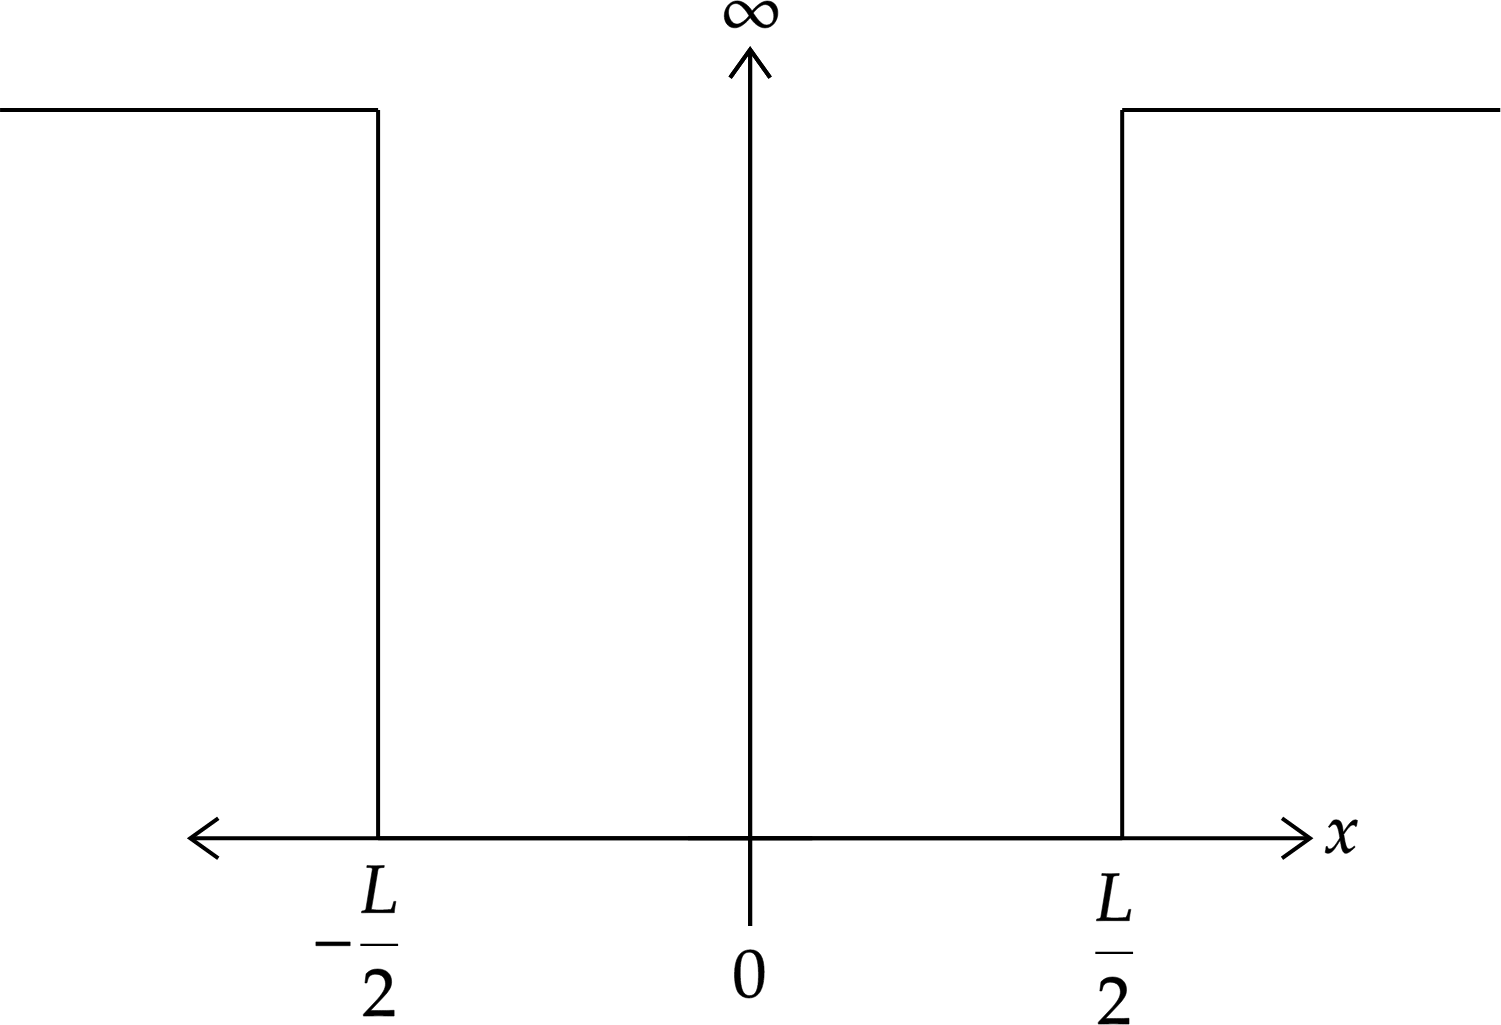
\includegraphics[scale=0.16]{diagram-20201209.png}
    \caption{$V(x)$ potentialet. Partiklet befinder sig i en uendeligt dyb ``tom dåse'' eller ``brønd''.}
    \label{fig:pot1}
\end{figure}
Vi begynder med en beskrivelse af et 1-dimensionelt potentiale $V(x)$ som set på Figur \ref{fig:pot1}. Potentialet er $\infty$ udenfor længden $L$, samt 0 indenfor. Dette kan beskrives således
\begin{align}
    V(x) = \begin{cases}
    0, & -\frac{L}{2} < x < \frac{L}{2} \\
    \infty, & x \leq -\frac{L}{2} \\
    \infty, & x \geq \frac{L}{2}
    \end{cases}
\end{align}
\subsection{Analytisk løsning af TISE}
I en positionsbasis kan man omskrive TISE fra (\ref{tise}) til
\begin{align}
     \label{awdb}
    \dv[2]{\psi}{x}+\frac{2m}{\hbar}(E-V(x))\psi = 0
\end{align}
Det er oplagt at inddele bølgefunktionen ind i tre regioner per potentialet. Jeg har denoteret bølgefunktionen venstre og højre region i ``væggen'' med hhv. 1 og 3 (ikke at forvirres med kvantetal). Indenfor væggene er bølgefunktionen kaldt $\psi_2$. Siden dette rimeligt kunstige potentiale er uendeligt kan et partikel selvfølgelig ikke befinde sig deri, da får jeg at $\psi_1=0$ og $\psi_3=0$. Man kan vise dette ved at løse (\ref{awdb}), hvori $V(x)$ i regionen sættes til et udefineret $\tilde V>E$, således at man kan tilnærme den faktiske $V$ som grænseværdi
\begin{align}
    \overbrace{
    \lim_{\tilde V\rightarrow \infty} \underbrace{\qty[\dv[2]{\psi_1}{x}-\frac{2m}{\hbar^2}(\tilde V-E)\psi_1]}_{\tilde \psi_1}}^{\psi_1} = 0
\end{align}
Denne ligning er en andensorden linær homogen differentialligning. Som set i (\ref{constantodewithcoefficients}), er løsningen for indholdet af parentesen af formen
\begin{align}
    \tilde \psi_1 = Ae^{-kx}+Be^{kx}
\end{align}
Hvor $\displaystyle k = \sqrt{\frac{2m(\tilde V-E)}{\hbar^2}}$. Siden denne region er defineret for $x\leq-\frac{L}{2}$, kræves der at $\psi_1\in L^2(\mathbb R^-)$ som set i (\ref{l2}) for at dette skal repræsentere noget fysisk. Man kan løse dette ved at sætte $A=0$, da $Ae^{-kx}$ divergerer når $x\to -\infty$, hvorved man ender med $\tilde \psi_1=Be^{kx}$. Nu kan man løse grænseværdien som
\begin{align}
    \psi_1 = \lim_{\tilde V\to \infty } Be^{kx} = 0
\end{align}
Lignende kan det omvendte vises for at $\psi_3=0$. Siden $V=0$ for $\psi_2$, refererer jeg til (24) for at få en løsning af formen
\begin{align}
\label{mid}
    \psi_2 &= Ae^{ikx}+Be^{-ikx}
\end{align}
Hvor $\displaystyle k = \sqrt{\frac{2mE}{\hbar^2}}$. Den totale bølgefunktion $\psi$ skal selvfølgelig være kontinuer, da kræver jeg at
\begin{align}
\label{betingelsea}
    \psi_1\qty(-\frac{L}{2})=\psi_2\qty(-\frac{L}{2})=0
\end{align}
samt at
\begin{align}
    \psi_3\qty(\frac{L}{2})=\psi_2\qty(\frac{L}{2})=0
\end{align}
Jeg omskriver (\ref{mid}) til at være
\begin{align}
    \psi_2 = A\cos(kx)+B\sin(kx)
\end{align}
Jeg undersøger nu hvor denne nulfaktor skal komme fra ved $x=+L/2,-L/2$. Antager man at den skal opstå fra $\sin(kx)$ kræves der at $kx=0$ ved f.eks $x=L/2$. Det er muligt såfremt at 
\begin{align}
\label{forstelso}
    k=\frac{n\pi}{L},\quad n=0,~\pm~2,~\pm 4,\dots
\end{align} I dette tilfælde kræves der at $A=0$. Gør man det samme med $\cos(kx)$ finder man en række løsninger af samme form som (\ref{forstelso}), hvori $n$ er alle ulige naturlige tal. Dette efterlader os med en række løsninger for bølgefunktionen
\begin{align}
    \psi_n = \begin{cases}
    A\sin\qty(\frac{n\pi x}{L}) & n=\pm2,~\pm 4,\dots \\
    B\cos\qty(\frac{n\pi x}{L}) & n=\pm1,~\pm 3,\dots
    \end{cases}
\end{align}
Man kan kort konkludere at $A=B$, samt finde normaliseringsfaktoren som
\begin{align}
\begin{split}
    \braket{\psi_n}{\psi_n} &= A \int_{-\frac{L}{2}}^{\frac{L}{2}} \sin^2\qty(\frac{n\pi x}{L})~dx=1 \\
    A &= \sqrt{\frac{2}{L}}
\end{split}
\end{align}
Man kan udlede energiegenværdierne $E_n$ fra relationen
\begin{align}
    k = \sqrt{\frac{2mE_n}{\hbar^2}} &= \frac{n\pi}{L}
\end{align}
da får man
\begin{align}
    E_n = \frac{\hbar^2}{2m}k^2_n = \frac{\hbar^2\pi^2n^2}{2mL^2}
\end{align}

Med udgangspunktet i TDSE fra (\ref{eq:schr}) kan jeg nu konstruere en tidsudvikling, også kaldt en stationær tilstand. Dette ligger i en antagelse af separation af variable som
\begin{align}
    \psi(x,t) = \hat K(t) \ket{\psi(x)}
\end{align}
For at opfylde TDSE, får man da løsningen
\begin{align}
    \psi_n(x,t) = A\psi_n(x)e^{-iE_nt/\hbar}
\end{align}
Enhver linær kombination $\Psi$ vil også befinde sig i $\mathcal H$, da er de også løsninger
\begin{align}
    \Psi = \sum_{n=1}^\infty c_nA\psi_n(x)e^{-iE_nt/\hbar}
\end{align}

\section{Hydrogenatomet}
\subsection{Potentialenergi}
Et Hydrogenlignende atom er ethvert atom der består af ét elektron samt et eller flere protoner. Problemet jeg undersøger har med at gøre to ladninger, hhv. $-e$ og $+e$, samt to masser $m_e$ og $M$ som korresponderer til hhv. elektronet og protonet. Den reducerede masse $\mu = \frac{m_eM}{m_e+M}$. Fra Coulomb's lov, får man
\begin{align}
    V(r) = \frac{-e^2}{4\pi \epsilon_0 r}
\end{align}
Hvilket beskriver potentialenergien mellem en elektronladning og atomkernen \parencite{griffiths}. Den kinetiske energi kan udledes fra den klassiske formalisme i.e.
\begin{align}
    T(q) = \frac{-\hbar^2}{2m}\pdv[2]{q} 
\end{align}
Hvilket giver
\begin{align}
    T(r) = \frac{-\hbar^2}{2\mu}\nabla^2
\end{align}
Dette udgør nu Hamiltonoperatoren $\hat H = \hat T+\hat V$ som
\begin{align}
\label{hydrogenhamil}
    \hat H = \frac{-\hbar^2}{2\mu}\nabla^2 - \frac{-e^2}{4\pi \epsilon_0 r}
\end{align}

\subsection{Analytisk løsning af TISE}
Fra (\ref{hydrogenhamil}) kan man opskrive TISE som
\begin{align}
\label{unextended}
    \qty[\frac{-\hbar^2}{2\mu}\nabla^2 - \frac{-e^2}{4\pi \epsilon_0 r}]\psi(r,\theta,\varphi)=E\psi(r,\theta,\varphi)
\end{align}
Man kan repræsentere $\nabla^2$ i sfæriske koordinater fra
\begin{align}
\nabla^2f &= \frac{1}{r^2} \frac{\partial}{\partial r} \left(r^2 \frac{\partial f}{\partial r} \right) + \frac{1}{r^2 \sin \theta} \frac{\partial}{\partial \theta} \left(\sin \theta \frac{\partial f}{\partial \theta} \right) + \frac{1}{r^2 \sin^2 \theta} \frac{\partial^2 f}{\partial \varphi^2},
\end{align}
Hvorfra man kan omskrive (\ref{unextended}) som
\begin{align}
    \begin{split}
         -\frac{\hbar^2}{2 \mu} \left[ \frac{1}{r^2} \frac{\partial}{\partial r} \left( r^2 \frac{\partial \psi}{\partial r} \right) + \frac{1}{r^2 \sin \theta} \frac{\partial}{\partial \theta} \left( \sin \theta \frac{\partial \psi}{\partial \theta} \right) + \frac{1}{r^2 \sin^2 \theta} \frac{\partial^2 \psi}{\partial \varphi^2} \right]\\
         - \frac{e^2}{4 \pi \epsilon_0 r} \psi = E \psi
    \end{split}
\end{align}
$E\psi$ kombineres med 
\begin{align}
\begin{split}
    \frac{1}{r^2}\frac{\partial}{\partial r}\left(r^2\frac{\partial\psi}{\partial r}\right)+\frac{1}{r^2\sin\theta}\frac{\partial}{\partial\theta}\left(\sin\theta\frac{\partial\psi}{\partial\theta}\right)+\frac{1}{r^2\sin^2\theta}\frac{\partial^2\psi}{\partial\varphi^2}\\+\frac{2\mu}{\hbar^2}\left(E+\frac{Ze^2}{4\pi\epsilon_0r}\right)\psi=0
\end{split}
\end{align}
Man kan antage, ved seperation af variable, af bølgefunktionen er et produkt af tre funktioner
\begin{align}
\label{opdeling}
    \psi(r, \theta, \varphi) = R(r)\Theta (\theta) \Phi (\varphi)
\end{align}
Siden ligningerne endnu er for indviklede, arbejder jeg til at begynde med, med vinkelfunktionerne i én, $A(\theta, \varphi) = \Theta(\theta)\Phi(\varphi)$. Siden radius- og vinkel er antaget uafhængigt, kan man lave en substitution hvor $\displaystyle \pdv{\psi}{\theta} = R\pdv{A}{\theta}$ og omvendt for afledede med respekt til $r$, således
\begin{align}
\begin{split}
    \frac{A}{r^2}\frac{\rm d}{{\rm d}r}\left(r^2\frac{{\rm d}R}{{\rm d}r}\right)+\frac{R}{r^2\sin\theta}\frac{\partial}{\partial\theta}\left(\sin\theta\frac{\partial A}{\partial\theta}\right)+\frac{R}{r^2\sin^2\theta}\frac{\partial^2A}{\partial\varphi^2}
    \\+\frac{2\mu}{\hbar^2}\left(E+\frac{Ze^2}{4\pi\epsilon_0r}\right)RA=0\qquad
\end{split}
\end{align}
Det næste mål er separere $R$ og $A$ såvidt muligt. $1/r^2$ er en gengående faktor som man kan fjerne ved multiplikation således
\begin{align}
\begin{split}
    A\frac{\rm d}{{\rm d}r}\left(r^2\frac{{\rm d}R}{{\rm d}r}\right)
    +\frac{R}{\sin\theta}\frac{\partial}{\partial\theta}\left(\sin\theta\frac{\partial A}{\partial\theta}\right)
    +\frac{R}{\sin^2\theta}\frac{\partial^2A}{\partial\varphi^2}
    \\
    +\frac{2\mu}{\hbar^2}r^2\left(E+\frac{Ze^2}{4\pi\epsilon_0r}\right)RA=0\qquad
\end{split}
\end{align}
Lignende kan man dividere med $RA$ for at få
\begin{align}
    \begin{split}
        \frac{1}{R}\frac{\rm d}{{\rm d}r}\left(r^2\frac{{\rm d}R}{{\rm d}r}\right)
        +\frac{1}{A\sin\theta}\frac{\partial}{\partial\theta}\left(\sin\theta\frac{\partial A}{\partial\theta}\right)
        +\frac{1}{A\sin^2\theta}\frac{\partial^2A}{\partial\varphi^2}
        \\
        +\frac{2\mu r^2}{\hbar^2}\left(E+\frac{Ze^2}{4\pi\epsilon_0r}\right)
        =0\qquad.
    \end{split}
\end{align}
Læg mærke til at de to yderste dele afhænger af $r$, mens de inderste afhænger af vinklerne (polær og azimut), som set forneden
\begin{align}
    \begin{split}
        \underbrace{\frac{1}{R}\frac{\rm d}{{\rm d}r}\left(r^2\frac{{\rm d}R}{{\rm d}r}\right)
        +\dots+\frac{2\mu r^2}{\hbar^2}\left(E+\frac{Ze^2}{4\pi\epsilon_0r}\right)}_{(r)}
        =0\qquad.
        \\
        \dots
        +\overbrace{\frac{1}{A\sin\theta}\frac{\partial}{\partial\theta}\left(\sin\theta\frac{\partial A}{\partial\theta}\right)
        +\frac{1}{A\sin^2\theta}\frac{\partial^2A}{\partial\varphi^2}}^{(\theta, \varphi)}+\dots
        =0\qquad.
    \end{split}
\end{align}
Hvis at disse dele tilsammen skal være lig 0, kræver det at de balancerer hinanden med en separationskonstant $K$. Dette betyder man kan få to ligninger af formen
\begin{subequations}
\begin{align}
\label{radi}
    \frac{\rm d}{{\rm d}r}\left(r^2\frac{{\rm d}R}{{\rm d}r}\right)+\frac{2\mu r^2}{\hbar^2}\left(E+\frac{Ze^2}{4\pi\epsilon_0r}\right)R-KR=0
\end{align}
og for delen afhængig af vinklerne,
\begin{align}
\label{angu}
    \frac{1}{\sin\theta}\frac{\partial}{\partial\theta}\left(\sin\theta\frac{\partial Y}{\partial\theta}\right)+\frac{1}{\sin^2\theta}\frac{\partial^2Y}{\partial\varphi^2}+KA=0
\end{align}
Fra (\ref{opdeling}), opdeler jeg $A(\theta, \varphi)$ op i funktioner afhængige af hhv. polær og azimut vinklerne, ved substitution i (\ref{angu}) således
\end{subequations}
\begin{align}
    \frac{\Phi}{\sin\theta}\frac{\rm d}{{\rm d}\theta}\left(\sin\theta\frac{{\rm d}\Theta}{{\rm d}\theta}\right)+\frac{\Theta}{\sin^2\theta}\frac{{\rm d}^2\Phi}{{\rm d}\varphi^2}+K\Phi\Theta=0
\end{align}
Dividerer man med $\Phi$, ganger med $\sin^2 \theta$ og dividerer med $\Theta$ kan man opdele de forskellige variable i forskellige dele. Derved får man følgende
\begin{align}
    \overbrace{\frac{\sin\theta}{\Theta}\frac{\rm d}{{\rm d}\theta}\left(\sin\theta\frac{{\rm d}\Theta}{{\rm d}\theta}\right)}^{(\theta)}
    +\underbrace{\frac{1}{\Phi}\frac{{\rm d}^2\Phi}{{\rm d}\varphi^2}}_{(\varphi)}
    +\overbrace{K\sin^2\theta}^{(\theta)}=0
\end{align}
Som før, skal disse dele balancere hinanden til 0, per en separationskonstant $C$. Igen får man to ligninger, den første afhængig af $\theta$
\begin{subequations}
\begin{align}
\label{thetasol}
    \frac{\sin\theta}{\Theta}\frac{\rm d}{{\rm d}\theta}\left(\sin\theta\frac{{\rm d}\Theta}{{\rm d}\theta}\right)+K\sin^2\theta-C=0
\end{align}
og en afhængig af $\varphi$ (ganget med $\Phi$)
\begin{align}
\label{phisol}
    \frac{{\rm d}^2\Phi}{{\rm d}\varphi^2}+C\Phi=0
\end{align}
\end{subequations}
(\ref{phisol}) kan som redegjort for i (\ref{constantodewithcoefficients}) løses generelt med (husk at $C=m^2$, som vist) 
\begin{align}
    \Phi(\varphi) = \alpha e^{im\varphi}+\beta e^{-im\varphi}
\end{align}
$m$ er igen diskret\footnote{$m$ opstår siden grænsebetingelserne kræver at $\forall m\in \mathbb N$ skal bevare probablitetsstrukturen.}, og $\beta=0$. $m$ er det første kvantetal jeg har specificeret i denne løsning. Flere vil følge. Ved løsningen af (\ref{phisol}), fandt man $C=m^2$ - dette bruges i (\ref{thetasol}) således
\begin{align}
    \frac{\sin\theta}{\Theta}\frac{\rm d}{{\rm d}\theta}\left(\sin\theta\frac{{\rm d}\Theta}{{\rm d}\theta}\right)+K\sin^2\theta-m^2=0
\end{align}
Den kan omskrives til
\begin{align}
\label{az1}
    \frac{1}{\sin\theta}\frac{\rm d}{{\rm d}\theta}\left(\sin\theta\frac{{\rm d}\Theta}{{\rm d}\theta}\right)+\left(K-\frac{m^2}{\sin^2\theta}\right)\Theta=0
\end{align}
Bølgefunktionen kan omskrives fra en funktion af $\theta$ til en funktion af $\cos \theta$. Dvs. en substitution der lyder $Y(\cos \theta) = \Theta(\theta)$, hvilket betyder $\displaystyle \pdv{\theta} = -\sin \theta \pdv{x}$ hvor $x=\cos \theta$. Med dette kan man omskrive (\ref{az1}) til
\begin{align}
    \frac{1}{\sin\theta}(-\sin\theta)\frac{\rm d}{{\rm d}x}\left(\sin\theta(-\sin\theta)\frac{{\rm d}Y}{{\rm d}x}\right)+\left(K-\frac{m^2}{\sin^2\theta}\right)Y=0
\end{align}
Dette kan simplificeres ved at samle fællesfaktorerne til
\begin{align}
    \frac{\rm d}{{\rm d}x}\left(\sin^2\theta\frac{{\rm d}Y}{{\rm d}x}\right)+\left(K-\frac{m^2}{\sin^2\theta}\right)Y=0
\end{align}
Fra det trigonometriske identitet angivet i (\ref{trigidentity}) kan man lave substitutionen $\sin^2\theta = 1-x^2$ således\footnote{fra den forrige substitution $x=\cos^2\theta$}
\begin{align}
    \frac{\rm d}{{\rm d}x}\left((1-x^2)\frac{{\rm d}Y}{{\rm d}x}\right)+\left(K-\frac{m^2}{1-x^2}\right)Y=0
\end{align}
Vi kan til sidst udregne den første del som
\begin{align}
    \frac{\rm d}{{\rm d}x}\left((1-x^2)\frac{{\rm d}Y}{{\rm d}x}\right) = (1-x^2)\frac{{\rm d}^2Y}{{\rm d}x^2}-2x\frac{{\rm d}Y}{{\rm d}x}
\end{align}
Hvilket giver os
\begin{align}
    (1-x^2)\frac{{\rm d}^2Y}{{\rm d}x^2}-2x\frac{{\rm d}Y}{{\rm d}x}+\left(K-\frac{m^2}{1-x^2}\right)Y=0
\end{align}
Som specificeret i (\ref{legendrede}) er dette et Legendre polynomial differentialigning. Fra (\ref{legpoly}) får man generaliseringen (og den fundne vinkelfunktion $Y(\theta, \varphi)$)
\begin{align}
    Y_{\mathscr l,m}(\theta, \varphi)=(1-x^2)^{\frac{m}{2}}\left(a_0\sum_{n=0}^{\infty}\frac{a_{2n}}{a_0}x^{2n}+a_1\sum_{n=1}^{\infty}\frac{a_{2n+1}}{a_1}x^{2n+1}\right)
\end{align}
Kvantetallet $\mathscr l$ opstår i rekursionsformlen hvor $K=\mathscr l ( \mathscr l +1)$ ved konvergens
\begin{align}
    a_{n+2}=\frac{(n+m)(n+m+1)-\mathscr l(\mathscr l+1)}{(n+1)(n+2)}a_n
\end{align}
Kvantetallet $m$ er afhængig af $\mathscr l$, i at det kun kan antage værdier hvor $m\leq|\mathscr l|$. Vender man tilbage til radiusfunktionen i (\ref{radi}), kan man udregne første del som
\begin{align}
    \dv{r}\qty ( r^2 \dv{R}{r}) = r^2 \dv[2]{R}{r} + 2r\dv{R}{r}
\end{align}
Dette giver os
\begin{align}
    r^2\frac{{\rm d}^2R}{{\rm d}r^2}+2r\frac{{\rm d}R}{{\rm d}r}+\frac{2\mu r^2}{\hbar^2}\left(E+\frac{Ze^2}{4\pi\epsilon_0r}\right)R-\mathscr l(\mathscr l+1)R=0
\end{align}
Dividerer man med $r^2$ får man
\begin{align}
\label{whatbesubs}
    \frac{{\rm d}^2R}{{\rm d}r^2}
    +\frac{2}{r}\frac{{\rm d}R}{{\rm d}r}
    +\left(\frac{2\mu}{\hbar^2}\left(E+\frac{Ze^2}{4\pi\epsilon_0r}\right)
    -\frac{\mathscr l\left(\mathscr l+1\right)}{r^2}\right)R=0
\end{align}
Lader man $\lim_{r\to \infty} R(r)=0$, igen siden $R(r)\in L^2$, vil brøkene gå mod 0. Dette rejser også en lignende forventing: at radiusfunktionen kan skrives som et produkt af funktionerne
\begin{align}
    R(r) = R_{\infty}(r)F(r)
\end{align}
Lader man da $r\to \infty$ bliver reciprokkene 0 således
\begin{align}
    \frac{{\rm d}^2R_{\infty}}{{\rm d}r^2}+\frac{2\mu E}{\hbar^2}R_{\infty}=0
\end{align}
Igen finder man en løsning af formen
\begin{align}
    R_{\infty}(r)=\alpha e^{ikr}+\beta e^{-ikr}
\end{align}
Hvor $\displaystyle k=\sqrt{\frac{2\mu E}{\hbar^2}}$. På grund af elektronets ladning, vil løsningen være en hvor energien $E$ går mod $E_0<0$ når elektronet er i niveauer tættere på kernen. Da får man $\beta = 0$. 
\begin{align}
    R_\infty(r) = \alpha e^{-kr}
\end{align}
Hvor $k=\sqrt{-\frac{2\mu E}{\hbar^2}}$. Substituerer man nu tilbage i (\ref{whatbesubs}), får man en differentialligning der kan løses hvis $F$ ekspanderes til en potensrække således
\begin{align}
    R(r) = R_{\infty}(r) \sum^{\infty}_{u=0} b_ur^u
\end{align}
Der findes både rekursive og non-rekursive løsninger for $b_u$, dog gælder det for alle løsninger at deres konvergens afhænger af endnu et kvantetal, $n$.\footnote{En rekursiv løsning findes i \cite["The Hydrogen Atom"]{griffqm}} Da får man
\begin{align}
    R_{n\mathscr l}(r) = \alpha e^{-kr}b_0 e^{c_n}
\end{align}
Hvor $c_n=\frac{\mu e^2r}{2\pi \epsilon_0 \hbar^2 n}$. Ved energirelationen til $c_n$, får man følgende energiniveauer
\begin{align}
\label{hbaren}
    E_n = \frac{-\mu e^2r^2}{8 \pi^2 \epsilon_0^2 \hbar^2 n^2}
\end{align}
Løsningen på bølgefunktionen vil til sidst lyde
\begin{align}
    \psi_{n\mathscr l m}(r, \theta, \varphi) = C R_{n\mathscr l}(r) Y_{\mathscr l m}(\cos \theta) e^{im\varphi}
\end{align}
Hvorved $C$ kan findes ved $\braket{\psi_{n\mathscr l m}}{\psi_{n\mathscr l m}}=1$.

\subsection{I sammenligning med Rydbergformlen}
\subsubsection{Teoretiske forventninger}    
Man kan kort omskrive (\ref{hbaren}) hvor $h=\hbar 2\pi$ til
\begin{align}
\label{energies}
    E_n=-\frac{\mu e^4}{8\epsilon_0^2h^2n^2}
\end{align}
Bohr modellen angiver følgende antagelser
\begin{enumerate}
    \item Elektroner befinder sig i diskrete tilstande.
    \item Elektroner emitterer ikke radiation i disse stationære tilstande eller baner.
    \item Et elektron kan få eller tabe energi ved at ``hoppe'' fra et diskret kredsløb til en anden. Dette beskrives gennem Planck relationen, $\displaystyle \Delta E = E_2 - E_1 = h\nu $
\end{enumerate}
Til stor success lod denne model sig, baseret på et delvist klassisk mekanisk model for atomet, udregne til stor præcision den emitterede eller absorberede energier ved tilstandstransitioner. Før Bohr's model var Rydbergformlen også kendt per empirisk udledning. Genkald Rydbergformlen for brint
\begin{align}
    \frac{1}{\lambda} = R_H\qty(\frac{1}{n^2_f}-\frac{1}{n^2_i})
\end{align}
hvor $\lambda$ er bølgelængden på det absorberede eller emitterede foton, $n_i$ er initial energitilstanden og $n_f$ er den endelige energitilstand. $R_H$ er Rydbergkonstanten\footnote{Bemærk at ``Rydbergkonstanten'' her og flere andre steder refererer til Rydbergkonstanten \textit{for Hydrogen}. Den præcise udledte konstant er kaldt $R_\infty$ - ikke til at forveksles med radialfunktionen $R(r)$ eller $R_{\infty}(r)$.}, som er empirisk kendt til 
\begin{align}
    R_H^* \approx \mu \cdot R_{\infty}\pm 3\cdot 10^{-5} \s{m^{-1}}
\end{align}
eller udledt til
\begin{align}
    R_H = \frac{m_e Ze^4}{8h^2\epsilon_0^2}
\end{align}
per Bohr's model og udregninger \parencite{bohr}. Mine kvantemekanisk udledte energiniveauer (\ref{energies}) er konceptuelt identisk til Bohr's, til forskel af $Z$, hvor $Z$ angiver antallet af protoner i kernen. Havde jeg taget udgangspunkt i et vilkårligt antal protoner, var jeg ankommet til samme svar (da de kritiske funktioner kun har været afhængig af $r$, hvorefter linearitet har bevaret masse og ladning associeret med atomkernen). Rydbergformlen kan konstrueres ud af den udledte energisætning (\ref{energies}) ved at indsætte $\Delta n$ for energiniveauerne, da får man
\begin{align}
\label{rydb}
    \Delta E_{n_i,n_f} = \frac{\mu e^4}{8\epsilon_0^2h^2}\qty(\frac{1}{n^2_f}-\frac{1}{n^2_i})
\end{align}
\subsubsection{Eksempel: Balmer-linjerne}
Johann Balmer fandt i 1885, synlige emissions spektrallinjer associeret med Brintatomets emission.
\begin{figure}[!h]
    \centering
    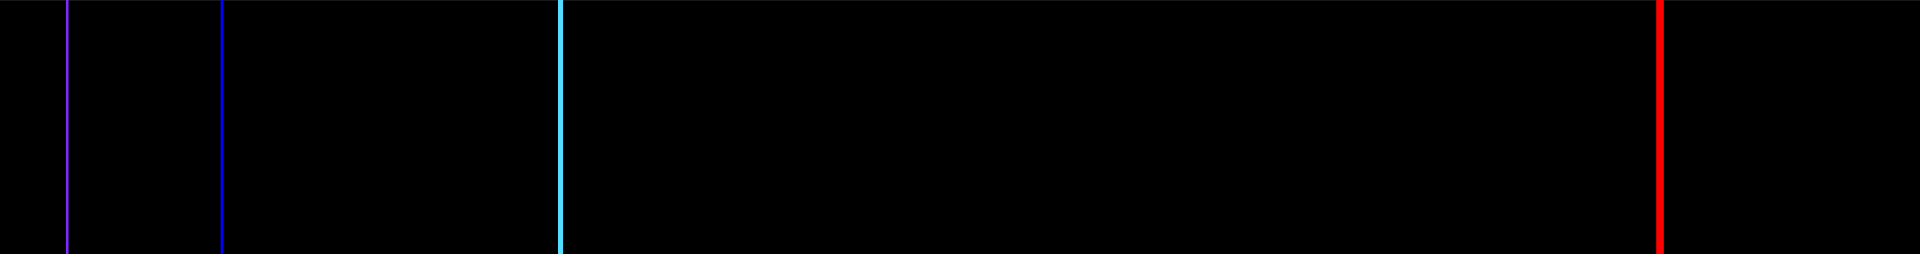
\includegraphics[width=\textwidth]{1920px-Emission_spectrum-H.svg.png}
    \caption{Fire synlige spektrallinjer.}
    \label{fig:my_label}
\end{figure}
Balmerlinjerne opstår ved skift fra en vilkårlig energitilstand til $n_f=2$ \parencite{wiese}. Dette data er præcist opstillet i Tabel \ref{tab:eksp}. 
\begin{table}[!h]
\label{tab:eksp}
    \centering
    \begin{tabular}{|l|cccccc}
    \hline\\
    $n_i$ & 3 & 4 & 5 & 6 & 7 & $\infty$ \\
    $\lambda$ (nm) & 656.3 & 486.1 & 434.0 & 410.2 & 397.0 & 364.6 
    \end{tabular}
    \caption{Eksperimentel data ved spektralanlyse \parencite{wiese}.}
\end{table}\\
Tabel 2 viser de teoretisk udledte Balmerlinjer hvor $\displaystyle n_i\to n_0$, gennem Planck-Einstein relationen $\displaystyle\lambda=\frac{hc}{\Delta E}$.
\begin{table}[!h]
\label{tab:teor}
    \centering
    \begin{tabular}{|l|cccccc}
        \hline\\
    $n_0$ & 3 & 4 & 5 & 6 & 7 & $\infty$ \\
    $\lambda$ (nm) & 656.1 & 486.1 & 433.9 & 410.1 & 397.0 & 364.5
    \end{tabular}
    \caption{Bølgelængder udregnet vha. (\ref{rydb}).}
\end{table}

Den gennemsnitlige relative fejlmargin $\delta u$ mellem eksperiment $n_i^*$ og teoretisk $n_i$ er fundet som
\begin{align}
    \delta u = \frac{1}{N}\sum^N_{k=1} \frac{\left| n_{i_k}^* - n_{i_k}\right|}{n_{i_k}}\cdot 100\% = 0.113\%
\end{align}
\subsubsection{Validitet af teoretiske forventninger}
De teoretisk regnede værdier stemmer overens med eksperimentelle data til en acceptabel grad i forhold til de givne antagelser. Den mest vitale antagelse kommer af at modellere systemet som et 1-legeme systemet, hvori protonkernen holdes immobilt samt center for referencerammen. Dette lader mig bruge den reducerede masse mellem protonet\footnote{Eller en (stort set) vilkårlig mængde ladninger} og elektronet. $m_e/M\simeq 1/2000$, hvilket betyder at $\mu \simeq m_e$. Systemet antages også nonrelativistisk per $ \frac{1}{2}mv^2 = \frac{p^2}{m}$. 

\section{Konklusion}
Den teoretiske undersøgelse havde til formål at sammenligne en nyere kvantemekanisk model med Bohr's originale atommodel, samt den tilhørende empiriske og udledte Rydbergformel. Forholdet blev kvantificeret ved sammenligning til to andre fremsætninger for Brint-Rydbergkonstanten $R_H$:
\begin{enumerate}
    \item Den originale empiriske Rydbergkonstant, $R^*_H$. 
    \item Bohr's semi-klassiske udledning af Rydbergkonstanten $R_H$.
\end{enumerate}
De teoretisk fundne energiniveauer i (\ref{energies}) viste sig identitiske til Bohr's fremsatte værdier, og da er den eneste forbedring i sikkerheden af værdierne i forhold til den empiriske Rydbergformel. Afsnit 5.3.3 viste at de givne antagelser har acceptabel fejlmargin ift. eksperimentelle værdier som blev produceret i afsnit 5.3.2.
\\\\
En konceptuel forbedring findes i fremsætningen af flere diskretiserede variable ved atomet, givet i de to andre kvantetal $\mathscr l$ og $m$. 

\newpage
\nocite{*}
\printbibliography

\end{document}
